\section{Mètode Intermig (M2/Orozco)}

El mètode intermig per resoldre el cub a cegues consta del mètode M2 per les arestes i l'Orozco per les cantonades.
El mètode M2, que com ja ho diu el seu nom es basa en el moviment M2, que és el moviment de la capa del mig del cub 2 vegades, a més a més, el buffer és UK (Aresta )

\begin{figure}[!ht]
    \centering
    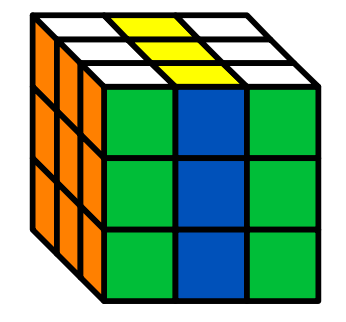
\includegraphics[width=5cm]{img/cubes/m2.png}
    \caption{Exemple de Moviment M2}
\end{figure}
    
Aquest mètode intercanvia les peces d'una manera peculiar, ja que ha de fer dues vegades M2 per tornar a l'estat original i canviar dues peces. Per exemple, fas primer la seqüència Y que col·loca la peça al lloc d'intercanvi, després fas la seqüència X que en aquesta cas és M2 i després fas Y' per retornar la peça intercanviada. Un cop fet això s'han canviat dues peces però el cub no queda igual que abans perquè hem de tornar a fer un intercanvi, aquest segon intercanvi ha de ser amb una seqüència Z X Z' perquè hem d'intercanviar una peça que no sigui la mateixa.\\\\Exemple d'intercanvi d'arestes L i V:

\begin{figure}[!ht]
    \centering
    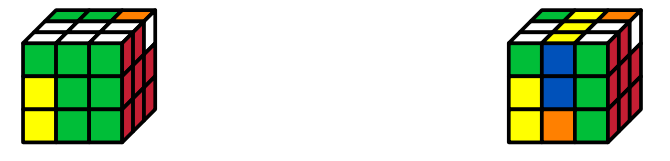
\includegraphics[width=9cm]{img/cubes/sec-1.png}
    \caption{Secuencia Y (Esquerra) i Y X (Dreta)}
\end{figure}

\begin{figure}[!ht]
    \centering
    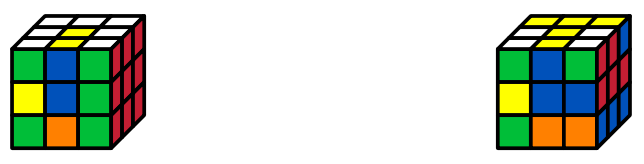
\includegraphics[width=9cm]{img/cubes/sec-2.png}
    \caption{Secuencia Y X Y' (Esquerra) i Y X Y'Z (Dreta)}
\end{figure}

\begin{figure}[!ht]
    \centering
    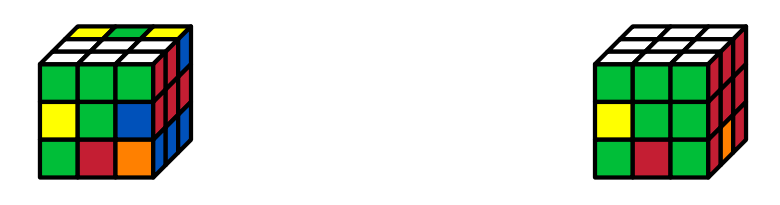
\includegraphics[width=9cm]{img/cubes/sec-3.png}
    \caption{Secuencia Y X Y'Z'X (Esquerra) i Y X Y'Z X Z' (Dreta)}
\end{figure}

Llavors així és com es canviarien dues arestes amb el mètode M2, en aquest cas L i V. El mètode té els casos de la taula \ref{fig:taula-m2}.

\begin{table}[h]
    \begin{minipage}{.5\linewidth}
        \centering
        \begin{tabular}{|c|c|}
            \hline
            A & M2 \\
            \hline
            B & R' U R U' M2 U R' U' R \\
            \hline
            C & U2 M' U2 M' \\
            \hline
            D & L U' L' U M2 U' L U L'  \\
            \hline
            E & B L' B' M2 B L B'  \\
            \hline
            F & B L2 B' M2 B L2 B' \\
            \hline
            G & B L B' M2 B L' B' \\
            \hline
            H & L B L' B' M2 B L B' L' \\
            \hline
            I & D M' U R2 U' M U R2 U' D' M2 \\
            \hline
            J & U R U' M2 U R' U' \\
            \hline
            K & Posició d'intercanvi \\
            \hline
            L & U' L' U M2 U' L U \\
            \hline 
        \end{tabular}
    \end{minipage}
    \begin{minipage}{.5\linewidth}
        \centering
        \begin{tabular}{|c|c|}
            \hline
             M & B' R B M2 B' R' B \\
             \hline
             N & R' B' R B M2 B' R' B R  \\
             \hline
             O & B' R' B M2 B' R B \\
             \hline
             P & B' R2 B M2 B' R2 B \\
             \hline
             Q & U B' R U' B (M2) B' U R' B U' \\
             \hline
             R & U' L U M2 U' L' U \\
             \hline
             S & M2' D U R2 U' M' U R2 U' M D' \\
             \hline
             T & U R' U' M2 U R U'  \\
             \hline
             U & Posició d'intercanvi \\
             \hline
             V & U R2 U' M2 U R2 U' \\
             \hline
             W & M U2 M U2  \\
             \hline
             X & U' L2 U M2 U' L2 U \\
             \hline 
        \end{tabular}
    \end{minipage} 
    \caption{Casos del Mètode M2}
    \label{fig:taula-m2}
\end{table}


\subsection{Mètode d'execució per les Cantonades}

El mètode orozco, utlitza un sistema similar al M2, ja que fa les seqüències Y X Y'X' i Z A Z' A' però en aquest cas la seqüència Z és diferent perquè es troba al segon lloc. De manera simple, si a la memorització tens la lletra en segon lloc has de fer l'algoritme alternatiu.
Els casos d'orozco són els de la taula \ref{fig:taula-orozco}

\begin{table}[!h]
    \begin{minipage}{.5\linewidth}
        \centering
        \begin{tabular}{|c|c|} 
            \hline
            \textbf{AB} & Basic A Perm \\
            \hline
            \textbf{DB} & U' (A Perm) U \\
            \hline
            \textbf{EB} & [R: [R D R', U]] \\
            \hline
            \textbf{FB} & [R': [U', R' D' R]] \\
            \hline
            \textbf{GB} & [U, R' D R] \\
            \hline
            \textbf{HB} & [R D' R', U'] \\
            \hline
            \textbf{IB} & [R: [R D R', U2]] \\
            \hline
            \textbf{KB} & [D': [U, R' D R]] \\
            \hline
            \textbf{LB} & [D: [U, R' D' R]] \\
            \hline
            \textbf{OB} & [R D R', U'] \\
            \hline
            \textbf{PB} & [U, R' D' R] \\
            \hline
            \textbf{RB} & [R': [U2, R' D' R]] \\
            \hline
            \textbf{SB} & [U, R' D2 R] \\
            \hline
            \textbf{TB} & [D: [R D' R', U']] \\
            \hline
            \textbf{UB} & [x': [R U R', D2]] \\
            \hline
            \textbf{VB} & [D' x': [R U R', D2]] \\
            \hline
            \textbf{WB} & [D x: [D2, R' U' R]] \\
            \hline
            \textbf{XB} & [x: [D2, R' U' R]] \\
            \hline 
        \end{tabular}
    \end{minipage}
    \begin{minipage}{.5\linewidth}
        \centering
        \begin{tabular}{|c|c|}
            \hline
            \textbf{BA} & Reverse A Perm \\
            \hline
            \textbf{BD} & U' (Reverse A Perm) U \\
            \hline
            \textbf{BE} & [R: [U, R D R']] \\
            \hline
            \textbf{BF} & [R': [R' D' R, U']] \\
            \hline
            \textbf{BG} & [R' D R, U] \\
            \hline
            \textbf{BH} & [U', R D' R'] \\
            \hline
            \textbf{BI} & [R: [U2, R D R']] \\
            \hline
            \textbf{BK} & [D': [R' D R, U]] \\
            \hline
            \textbf{BL} & [D: [R' D' R, U]] \\
            \hline
            \textbf{BO} & [U', R D R'] \\
            \hline
            \textbf{BP} & [R' D' R, U] \\
            \hline
            \textbf{BR} & [R': [R' D' R, U2]] \\
            \hline
            \textbf{BS} & [R' D2 R, U] \\
            \hline
            \textbf{BT} & [D: [U', R D' R']] \\
            \hline
            \textbf{BU} & [x': [D2, R U R']] \\
            \hline
            \textbf{BV} & [D' x': [D2, R U R']] \\
            \hline
            \textbf{BW} & [D x: [R' U' R, D2]] \\
            \hline
            \textbf{BX} & [x: [R' U' R, D2]] \\
            \hline 
        \end{tabular}
    \end{minipage} 
    \caption{Algorimtes orozco}
    \label{fig:taula-orozco}
\end{table}

A la columna de l'esquerra hi ha els corresponents a la primera lletra del parell i a la dreta els corresponents a la segona lletra del parell. \textit{A perm} és un cas del cub de rubik normal que es fa (R' U' R' D' R U' R' D R U R' D' R U R' D R2).
Cal tambe tenir en compte que els algoritmes estan una notació diferents perquè es vegi de millor forma al ser tants algoritmes. Funciona de la següent manera [A,B] = A,B,A',B'.

\begin{table}[h]
    \begin{minipage}{.5\linewidth}
        \centering
        \begin{tabular}{|c|c|}
            \hline
            \textbf{NB} & [U, R' D R D' R' D' R] \\
            \hline
            \textbf{QB} & [R' D R D' R' D' R, U] \\
            \hline
        \end{tabular}
    \end{minipage}
    \begin{minipage}{.5\linewidth}
        \centering
        \begin{tabular}{|c|c|}
            \hline
            \textbf{BN} & [R' D R D' R' D' R, U] \\
            \hline
            \textbf{BQ} & [U, R' D R D' R' D' R] \\
            \hline 
        \end{tabular}
    \end{minipage} 
    \caption{Excepcions del mètode}
\end{table}



Aquests algoritmes estan escrits en una notació\footnote{Manera d'escriure els algoritmes} diferenti [Y,X]. El fet que estigui entre claudators indica que s'ha de fer en l'ordre Y X Y' X'. És una mica més díficil de visualitzar però més fàcil a l'hora d'aplicar aquest mètode.
Exepmle d'intercanvi de dues cantonades P i H

\begin{figure}[!ht]
    \centering
    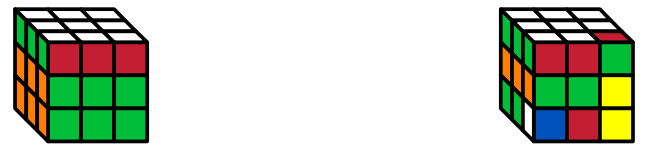
\includegraphics[width=9cm]{img/cubes/sec-4.png}
    \caption{Secuencia Y (Esquerra) i Y X (Dreta)}
\end{figure}

\begin{figure}[!ht]
    \centering
    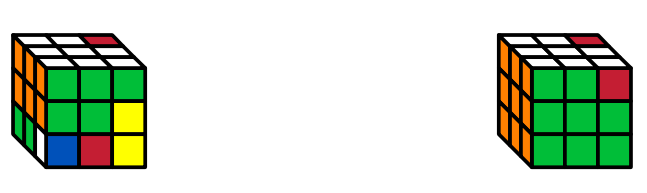
\includegraphics[width=9cm]{img/cubes/sec-5.png}
    \caption{Secuencia Y X Y' (Esquerra) i Y X Y' X'(Dreta)}
\end{figure}

\begin{figure}[!ht]
    \centering
    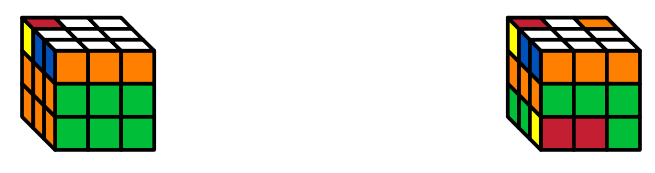
\includegraphics[width=9cm]{img/cubes/sec-6.png}
    \caption{Secuencia Y X Y' X' Z (Esquerra) i Y X Y' X' Z A(Dreta)}
\end{figure}

\begin{figure}[!ht]
    \centering
    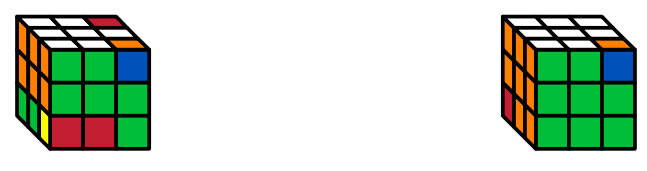
\includegraphics[width=9cm]{img/cubes/sec-7.png}
    \caption{Secuencia Y X Y' X' Z A Z' (Esquerra) i Y X Y' X' Z A Z' A'(Dreta)}
\end{figure}

Com a orientació [Y,X] i [Z,A] són a la taula d'algoritmes PB i BH.

\newpage
\large{Fins aquí el tutorial de 3BLD, espero que hagi sigut de fàcil comprensió i que t'hagi ajudat a resoldre el cub a cegues a les següents pàgines trobaràs les taules de memorització i dels algoritmes d'orozco i M2.}